\begin{activity} \label{8.1.Act1}
\ba
\item Let $s_n$ be the $n$th term in the sequence $1, 2, 3, \ldots$. 

Find a formula for $s_n$ and use appropriate technological tools to draw a graph of entries in this sequence by plotting points of the form $(n,s_n)$ for some values of $n$. Most graphing calculators can plot sequences; directions follow for the TI-84.
\begin{itemize}
\item In the MODE menu, highlight SEQ in the FUNC line and press ENTER.
\item In the Y= menu, you will now see lines to enter sequences. Enter a value for $n$Min (where the sequence starts), a function for $u(n)$ (the $n$th term in the sequence), and the value of $u_{n\text{Min}}$.
\item Set your window coordinates (this involves choosing limits for $n$ as well as the window coordinates XMin, XMax, YMin, and YMax.
\item The GRAPH key will draw a plot of your  sequence.
\end{itemize}
Using your knowledge of limits of continuous functions as $x \to \infty$, decide if this sequence $\{s_n\}$ has a limit as $n \to \infty$. Explain your reasoning.

\item Let $s_n$ be the $n$th term in the sequence $1, \frac{1}{2}, \frac{1}{3}, \ldots$. Find a formula for $s_n$. Draw a graph of some points in this sequence. Using your knowledge of limits of continuous functions as $x \to \infty$, decide if this sequence $\{s_n\}$ has a limit as $n \to \infty$. Explain your reasoning.

\item Let $s_n$ be the $n$th term in the sequence $2, \frac{3}{2}, \frac{4}{3}, \frac{5}{4}, \ldots$. Find a formula for $s_n$. Using your knowledge of limits of continuous functions as $x \to \infty$, decide if this sequence $\{s_n\}$ has a limit as $n \to \infty$. Explain your reasoning.

\ea
\end{activity}

\begin{smallhint}
\ba
	\item Small hints for each of the prompts above.
\ea
\end{smallhint}
\begin{bighint}
\ba
	\item Big hints for each of the prompts above.
\ea
\end{bighint}
\begin{activitySolution}
\ba
	\item By observation we see that a formula for $s_n$ is $s_n = n$. A plot of the first 50 points in the sequence is shown here.
%\begin{center} 
%\resizebox{!}{1.75in}{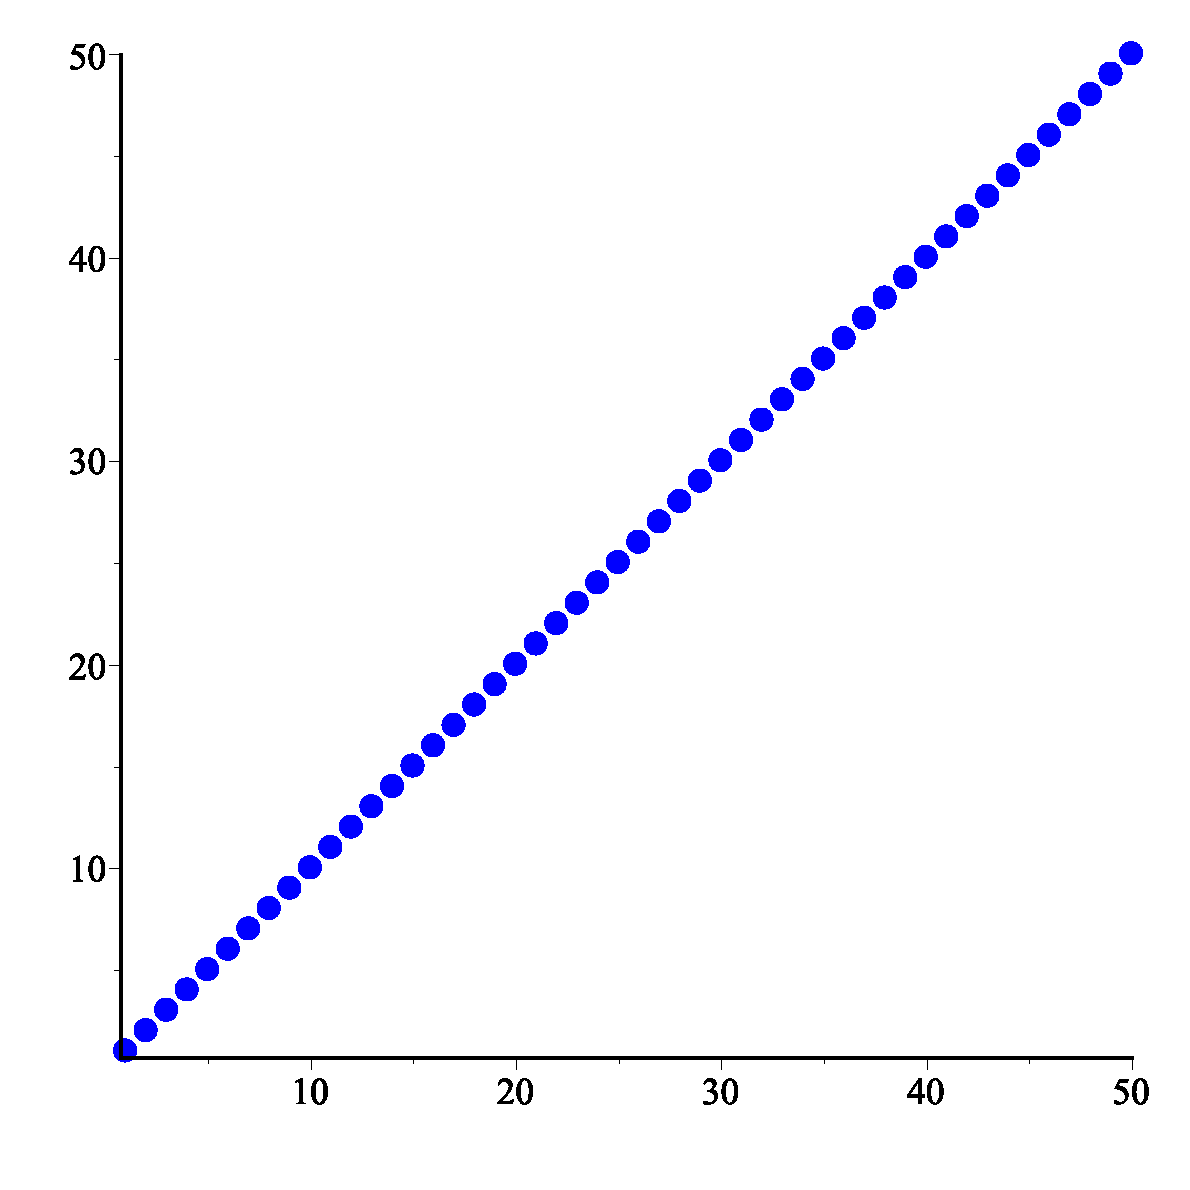
\includegraphics{figures/8_1_Sequence_n.eps}} 
%\end{center}
We recalling that a function $f$ has a limit $L$ at infinity if we can make the values of $f(x)$ as large as we want by choosing $x$ as large as we need. Since we can make the values of $n$ in our sequence as large as we want by choosing $n$ to be as large as we need, we suspect that this sequence does not have a limit as $n$ goes to infinity.

\item By observation we see that a formula for $s_n$ is $s_n = \frac{1}{n}$. A plot of the first 50 points in the sequence is shown here.
%\begin{center} \resizebox{!}{1.75in}{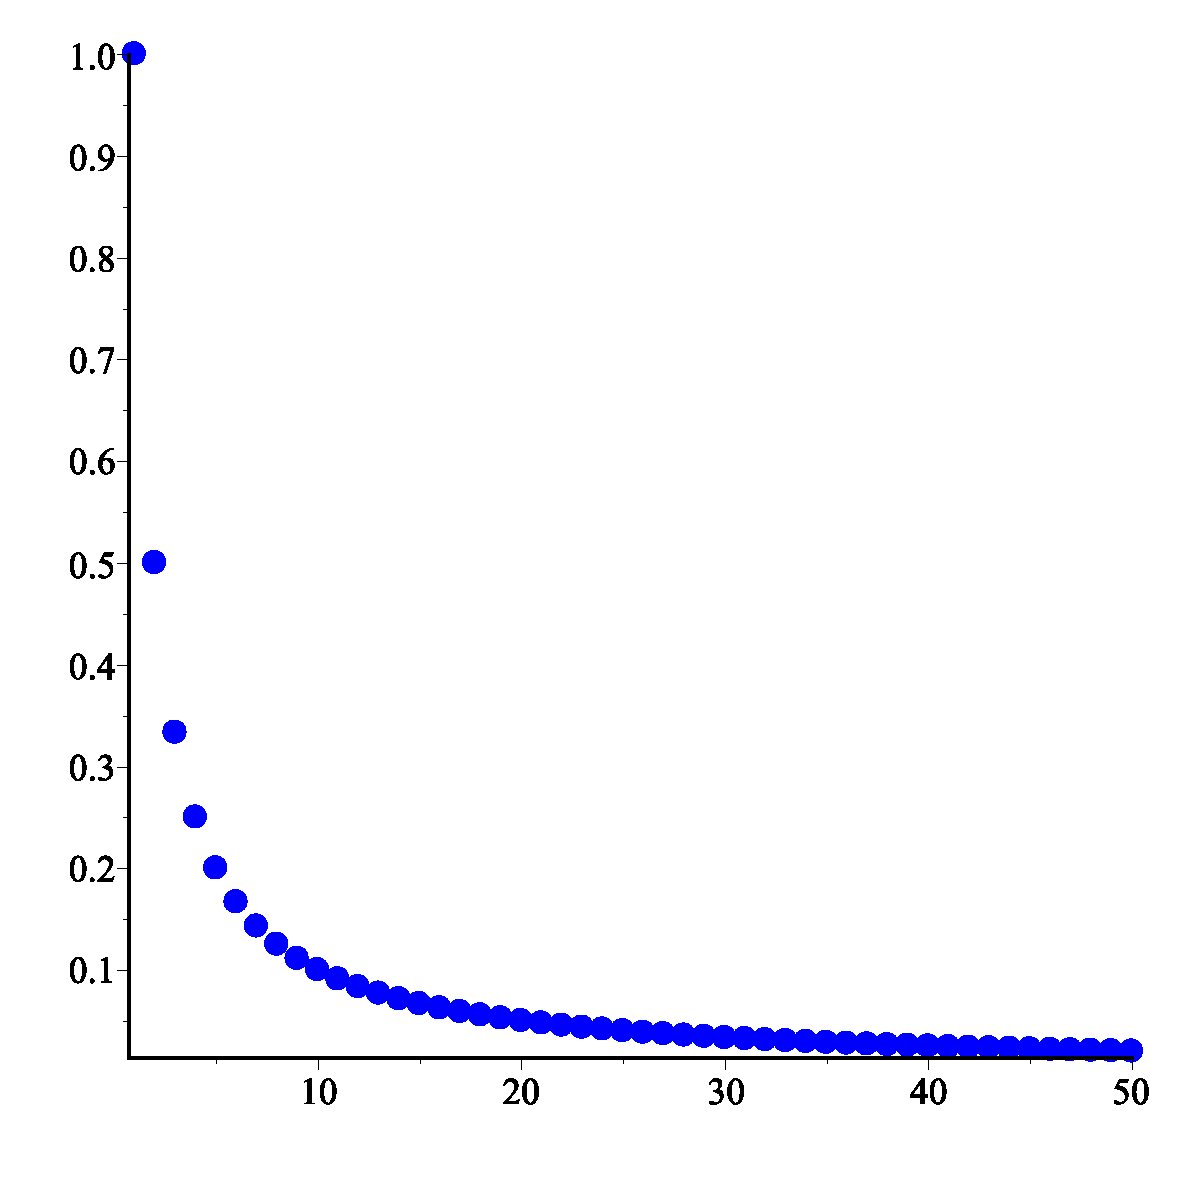
\includegraphics{figures/8_1_Sequence_1overn.eps}} \end{center}
Since we can make the values of $\frac{1}{n}$ in our sequence as close to 0 as we want by choosing $n$ to be as large as we need, we suspect that this sequence has a limit of 0 as $n$ goes to infinity.

\item Since the numerator is always 1 more than the denominator, a formula for $s_n$ is $s_n = \frac{n+1}{n}$. A plot of the first 50 points in the sequence is shown here.
%\begin{center} \resizebox{!}{1.75in}{\includegraphics{figures/8_1_Sequence_nplus1overn.eps}} \end{center}
Since we can make the values of $\frac{n+1}{n}$ in our sequence as close to 1 as we want by choosing $n$ to be as large as we need, we suspect that this sequence has a limit of 1 as $n$ goes to infinity.

\ea
\end{activitySolution}
\aftera 